\documentclass[a4paper]{article}
\usepackage[utf8]{inputenc}
\usepackage{amsthm, amsmath, mathtools, amssymb}
\usepackage[left=2cm,right=2cm,top=2cm,bottom=2cm]{geometry}
\usepackage[colorlinks,linkcolor=blue,citecolor=blue,urlcolor=blue]{hyperref}
\usepackage{array}
\usepackage[catalan,english]{babel}
\usepackage[affil-it]{authblk}
\usepackage{titlesec}
\usepackage[intlimits]{esint} % for more options on integrals.
\usepackage{physics}
\usepackage[hypcap=false]{caption}
\usepackage{subcaption}
\usepackage{multirow}
% \titleformat{\section}
%   {\normalfont\fontsize{13}{15}\bfseries}{\thesection}{1em}{}

\newcommand{\NN}{\ensuremath{\mathbb{N}}} % set of natural numbers
\newcommand{\ZZ}{\ensuremath{\mathbb{Z}}} % set of integers
\newcommand{\QQ}{\ensuremath{\mathbb{Q}}} % set of rationals
\newcommand{\RR}{\ensuremath{\mathbb{R}}} % set of real numbers
\newcommand{\CC}{\ensuremath{\mathbb{C}}} % set of complex numbers
\newcommand{\KK}{\ensuremath{\mathbb{K}}} % a general field

\newcommand{\vf}[1]{\boldsymbol{\mathrm{#1}}} % math style for vectors and matrices and vector-values functions (previously it was \*vb{#1} but this does not apply to greek letters)
\newcommand{\ii}{\mathrm{i}} % imaginary unit
\newcommand{\OO}{\mathrm{O}}

\newtheorem{theorem}{Teorema}
\newtheorem{prop}{Proposició}
\theoremstyle{definition}
\newtheorem{definition}{Definició}
\DeclareDocumentCommand\derivative{ s o m g d() }{ 
  % Total derivative
  % s: star for \flatfrac flat derivative
  % o: optional n for nth derivative
  % m: mandatory (x in df/dx)
  % g: optional (f in df/dx)
  % d: long-form d/dx(...)
    \IfBooleanTF{#1}
    {\let\fractype\flatfrac}
    {\let\fractype\frac}
    \IfNoValueTF{#4}
    {
        \IfNoValueTF{#5}
        {\fractype{\diffd \IfNoValueTF{#2}{}{^{#2}}}{\diffd #3\IfNoValueTF{#2}{}{^{#2}}}}
        {\fractype{\diffd \IfNoValueTF{#2}{}{^{#2}}}{\diffd #3\IfNoValueTF{#2}{}{^{#2}}} \argopen(#5\argclose)}
    }
    {\fractype{\diffd \IfNoValueTF{#2}{}{^{#2}} #3}{\diffd #4\IfNoValueTF{#2}{}{^{#2}}}\IfValueT{#5}{(#5)}}
} % differential operator
\DeclareDocumentCommand\partialderivative{ s o m g d() }{ 
  % Total derivative
  % s: star for \flatfrac flat derivative
  % o: optional n for nth derivative
  % m: mandatory (x in df/dx)
  % g: optional (f in df/dx)
  % d: long-form d/dx(...)
  \IfBooleanTF{#1}
    {\let\fractype\flatfrac}
    {\let\fractype\frac}
    \IfNoValueTF{#4}{
      \IfNoValueTF{#5}
      {\fractype{\partial \IfNoValueTF{#2}{}{^{#2}}}{\partial #3\IfNoValueTF{#2}{}{^{#2}}}}
      {\fractype{\partial \IfNoValueTF{#2}{}{^{#2}}}{\partial #3\IfNoValueTF{#2}{}{^{#2}}} \argopen(#5\argclose)}
    }
    {\fractype{\partial \IfNoValueTF{#2}{}{^{#2}} #3}{\partial #4\IfNoValueTF{#2}{}{^{#2}}}\IfValueT{#5}{(#5)}}
} % partial differential operator

\renewcommand{\labelenumii}{\alph{enumii})}

\title{\bfseries\large SEMINARI 2\\\vspace{0.25cm}Problema centre - focus i bifurcació de Hopf}

\author{Víctor Ballester Ribó\endgraf NIU:1570866}
\date{\parbox{\linewidth}{\centering
  Sistemes dinàmics\endgraf
  Grau en Matemàtiques\endgraf
  Universitat Autònoma de Barcelona\endgraf
  Gener de 2023}}

\setlength{\parindent}{0pt}
\begin{document}
\selectlanguage{catalan}
\maketitle
En aquest document ens dedicarem a estudiar l'estabilitat de l'origen en funció de paràmetres per a diferents sistemes diferencials així com el nombre d'òrbites periòdiques que poden néixer de l'origen en cada cas.
\section*{Exercici 1}
Considerem el sistema diferencial:
\begin{equation}\label{sis1}
  \left\{
  \begin{aligned}
    x' & =-y                    \\
    y' & =x + ay +bx^2+cx^3+x^4
  \end{aligned}
  \right.
\end{equation}
amb $a,b,c\in\RR$.

Observem d'entrada que si $a\ne 0$, l'origen és hiperbòlic i per tant és estable si $a<0$ i inestable si $a>0$. Pel cas $a=0$, fixem-nos que el sistema és Hamiltonià amb integral primera (definida en un entorn de l'origen): $$H=\frac{x^2}{2}+\frac{y^2}{2}+b\frac{x^3}{3}+c\frac{x^4}{4}+\frac{x^5}{5}$$
Per tant, com que el sistema rota al voltant de l'origen, aquest és un centre $\forall b,c \in\RR$.

Finalment notem que la divergència del sistema és $a$. I per tant si $a\ne 0$, el teorema de Bendixson ens assegura que no hi ha cicles límit al sistema per cap valor de $a,b,c\in\RR$, $a\ne 0$.
\newpage
\section*{Exercici 2}
Considerem el sistema diferencial:
\begin{equation}\label{sis2}
  \left\{
  \begin{aligned}
    x' & =ax-y+x^2     \\
    y' & =x + y^2+b xy
  \end{aligned}
  \right.
\end{equation}
amb $a,b\in\RR$.

El sistema té divergència $a$ a l'origen, que té signe constant si $a\ne 0$. Per tant, l'estabilitat de l'origen si $a\ne 0$ ve donada pel signe de $a$. Si $a>0$, l'origen és inestable; si $a<0$, és estable. Ara suposem $a=0$. La primera constant de Lyapunov és $L_1=-b/4$. Per tant, aquest cop l'estabilitat ve donada pel signe de $b$. Si ara suposem $a=b=0$, el sistema resultant
$$
  \left\{
  \begin{aligned}
    x' & =-y+x^2  \\
    y' & =x + y^2
  \end{aligned}
  \right.
$$
és simètric respecte el canvi $(x, y, t)\to(-y,-x,-t)$, que correspon a la simetria respecte la recta $x+y=0$. Com que el sistema rota en un entorn de l'origen, aquest és un centre. En resum, em obtingut els següents resultats:
$$\text{L'origen és }
  \begin{cases}
    \text{estable}   & \text{si } a < 0 \text{ o } a = 0, b>0  \\
    \text{inestable} & \text{si } a > 0  \text{ o } a = 0, b<0 \\
    \text{centre}    & \text{si } a = b= 0
  \end{cases}
$$
Per estudiar el nombre de cicles límit que neixen de l'origen fixem-nos que si $a=0$, podem escriure la funció de retorn en sèrie de potències respecte $L_1$ i factoritzar-la de la forma:
$$\Delta (\rho)=L_1\rho^3(1 + \OO(\rho^2))$$
que és un polinomi que no té zeros per $\rho\gtrsim 0$ i $b\ne 0$. Ara suposem $a \ne 0$. El coeficient $L_1$ (en polars) s'escriu en sèrie de potències com $$L_1=-\frac{b\pi}{4} + \OO(a)$$ i la resta de $L_n$, $n\geq 2$, s'anu\lgem en amb $L_1$. Per tant, si $b=0$ no podem tenir cicles límit bifurcant de l'origen perquè la correponent aplicació de retorn només tindria el primer terme. Ara bé, si $b\ne 0$ aleshores podem escriure l'aplicació de retorn com:
$$\Delta (\rho)=(L_0 - 1 ) \rho+ L_1\rho^3(1 + \OO(\rho^2))\simeq \rho\left[(\pi a +\OO(a^2)) + \left(-\frac{b\pi}{4}+ \OO(a)\right) \rho^2\right]$$ que té un únic zero positiu (que tendeix a zero quan $a\to 0$). Per tant, només tindrem un únic cicle límit bifurcant de l'origen, que és el corresponent al de Hopf.
\begin{figure}[ht]
  \centering
  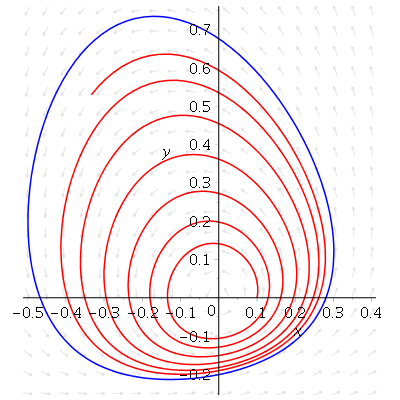
\includegraphics[width=0.49\linewidth]{Images/ex2-lc.png}
  \caption{Cicle límit de Hopf del sistema \eqref{sis2} amb $a=0.1$ i $b=3$}
\end{figure}

\newpage
\section*{Exercici 3}
Considerem el sistema diferencial:
\begin{equation}\label{sis3}
  \left\{
  \begin{aligned}
    x' & =-y+xy+x^2      \\
    y' & =x + ax^2 +by^2
  \end{aligned}
  \right.
\end{equation}
amb $a,b\in\RR$.

Les tres primeres constants de Lyapunov d'aquest sistema són les següents:
$$L_1=\frac{1-2a}{4}\qquad L_2=\frac{4b^3-7b-1}{16}\qquad L_3 = 0$$
on per calcular cadascuna hem assumit que les anteriors eren zero. Recordem que, com que el sistema és quadràtic, no cal calcular-ne més, ja que totes les següents també seran 0. L'estabilitat, doncs, la tenim determinada excepte per quan $a=1/2$ i $b$ satisfà $4b^3-7b-1=0$. Les arrels d'aquest polinomi s'exposen a continuació:
\begin{equation}\label{eqbs}
  b_1=-1.244644286...\quad b_2=-0.1445842733...\quad b_3=1.389228559...
\end{equation}

\begin{figure}[ht]
  \centering
  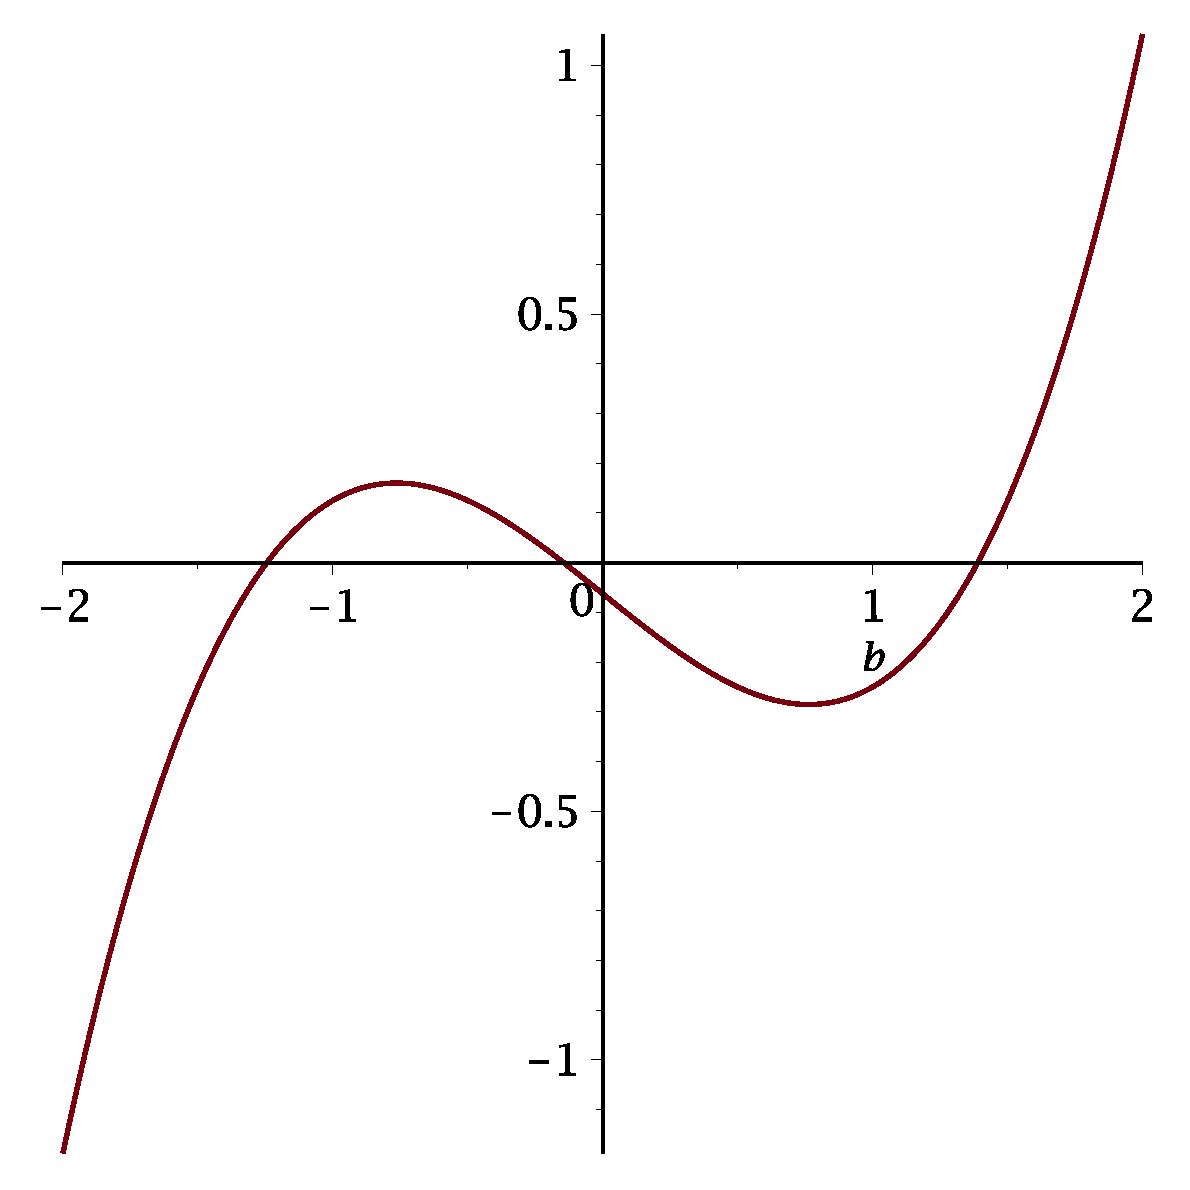
\includegraphics[width=0.49\linewidth]{Images/ex3.eps}
  \caption{Polinomi $4b^3-7b-1$}
\end{figure}

Pel teorema de Bautin, podem concloure que en aquests darrers tres casos tindrem centres a l'origen. Així doncs tenim que:
$$\text{L'origen és }
  \begin{cases}
    \text{estable}   & \text{si } a > 1/2 \text{ o } a = 1/2, b<b_1 \text{ o }  a = 1/2, b_2b<b_3  \\
    \text{inestable} & \text{si } a < 1/2 \text{ o } a = 1/2, b_1<b<b_2 \text{ o }  a = 1/2, b>b_3 \\
    \text{centre}    & \text{si } a = 1/2, b=b_1, b_2, b_3
  \end{cases}
$$

Observem que per $a=1/2$ i $b$ proper a als punts crítics de \eqref{eqbs} per un argument similar al de l'exercici 2, deduïm que no pot haver cicles límit. Ara bé, si $a\simeq 1/2$, aleshores: $$\Delta(\rho)\simeq L_1\rho^3+L_3\rho^5$$
que té un zero positiu si $b$ no és cap dels punts punts crítics de \eqref{eqbs}. Per tant, només podem assegurar l'existència d'un cicle límit.

\newpage
\section*{Exercici 4}
Considerem el sistema diferencial:
\begin{equation}\label{sis4}
  \left\{
  \begin{aligned}
    x' & =ax-y-9x^2+4xy+by^2   \\
    y' & =x +ay+2x^2-7xy -2y^2
  \end{aligned}
  \right.
\end{equation}
amb $a,b\in\RR$.

La divergència del sistema a l'origen és $a$. Per tant, l'estabilitat ve donada per el signe de $a$ si $a\ne 0$. Ara suposem $a=0$. Els tres primers coeficients de Lyapunov són els següents:
$$L_1=0\qquad L_2=-\frac{125\pi(b-4)(b-9)}{12}\qquad L_3 = 0$$
En sèrie de potències respecte la traça tenen la següent forma:
$$L_0=1+2\pi a \OO(a^2)\qquad L_1=\frac{\pi(10b^2+67b-114)}{24}a+\OO(a^2)\qquad L_2=-\frac{125\pi(b-4)(b-9)}{12} +\OO(a)$$
Per tant, deduïm que:
$$\text{L'origen és }
  \begin{cases}
    \text{estable}   & \text{si } a < 0 \text{ o } a = 0, b<4 \text{ o }  a = 0, b>9 \\
    \text{inestable} & \text{si } a > 0 \text{ o } a = 0, 4<b<9                      \\
    \text{centre}    & \text{si } a = 0, b=4,9
  \end{cases}
$$
Una observació és que per $a = 0$ i $b=4, 9$ el sistema és Darboux integrable perquè té cobres algebraiques de grau 2 i 3 en el primer cas i corbes algebraiques de grau 1 i 2 en el segon que donen lloc a una integral primera ben definida a l'origen.

Estudiem ara el nombre de cicles límit que poden néixer de l'origen. De nou, de forma anàloga als exercicis anteriors si $b=4$ o $b=9$ no podem tenir bifurcació de Hopf ja que per $a=0$ tenim un centre. Per tant suposem que $b\ne 4,9$. Llavors l'aplicació de retorn és:
$$\Delta(\rho)\simeq \rho\left[2\pi a + \frac{\pi(10b^2+67b-114)}{24}a\rho^2-\frac{125\pi(b-4)(b-9)}{12}\rho^4\right]$$
Per tant, com que $b\ne 4,9$:
$$\Delta(\rho)=0\iff \rho^2 - \frac{(10b^2+67b-114)a}{250(b-4)(b-9)}\rho-\frac{24a}{125(b-4)(b-9)} = 0$$
Però això només pot tenir un zero bifurcant de l'origen quan $a\to 0$. Per tant, només podem tenir un cicle límit.

\newpage
\section*{Exercici 5}
Considerem el sistema diferencial:
\begin{equation}\label{sis5}
  \left\{
  \begin{aligned}
    x' & = 6\varepsilon x-24ax^2-18xy-3\varepsilon+24x \\
    y' & =2(3y-2)(3y+\varepsilon)
  \end{aligned}
  \right.
\end{equation}
amb $a>0$ i $\varepsilon\in\RR$. En aquest cas se'ns demana estudiar l'estabilitat de tots els equilibris.

Els equilibris que tenim són els següents:
$$z_\pm^1= \left(\frac{\varepsilon+2\pm\sqrt{-8a\varepsilon+{(\varepsilon+2)}^2}}{8a},\frac{2}{3}\right) \quad z_\pm^2= \left(\frac{\varepsilon+2\pm\sqrt{-2a\varepsilon+{(\varepsilon+2)}^2}}{4a},-\frac{\varepsilon}{3}\right)$$
Els valors propis de les diferencials a cada punt són els següents:
\begin{align*}
  \sigma(D\vf{X}(z_\pm^1)) & =\left\{12+6\varepsilon, \mp6\sqrt{-8a\varepsilon+{(\varepsilon+2)}^2}\right\}     \\
  \sigma(D\vf{X}(z_\pm^2)) & =\left\{-(12+6\varepsilon), \mp12\sqrt{-2a\varepsilon+{(\varepsilon+2)}^2}\right\}
\end{align*}
Definim $f(a, \varepsilon)=-8a\varepsilon+{(\varepsilon+2)}^2$ i $g(a, \varepsilon) =-2a\varepsilon+{(\varepsilon+2)}^2$. Fixem-nos quan $f(a, \varepsilon)< 0$ perdrem dos punts d'equilibri i el mateix passa per $g(a,\varepsilon)$.
\begin{figure}[ht]
  \centering
  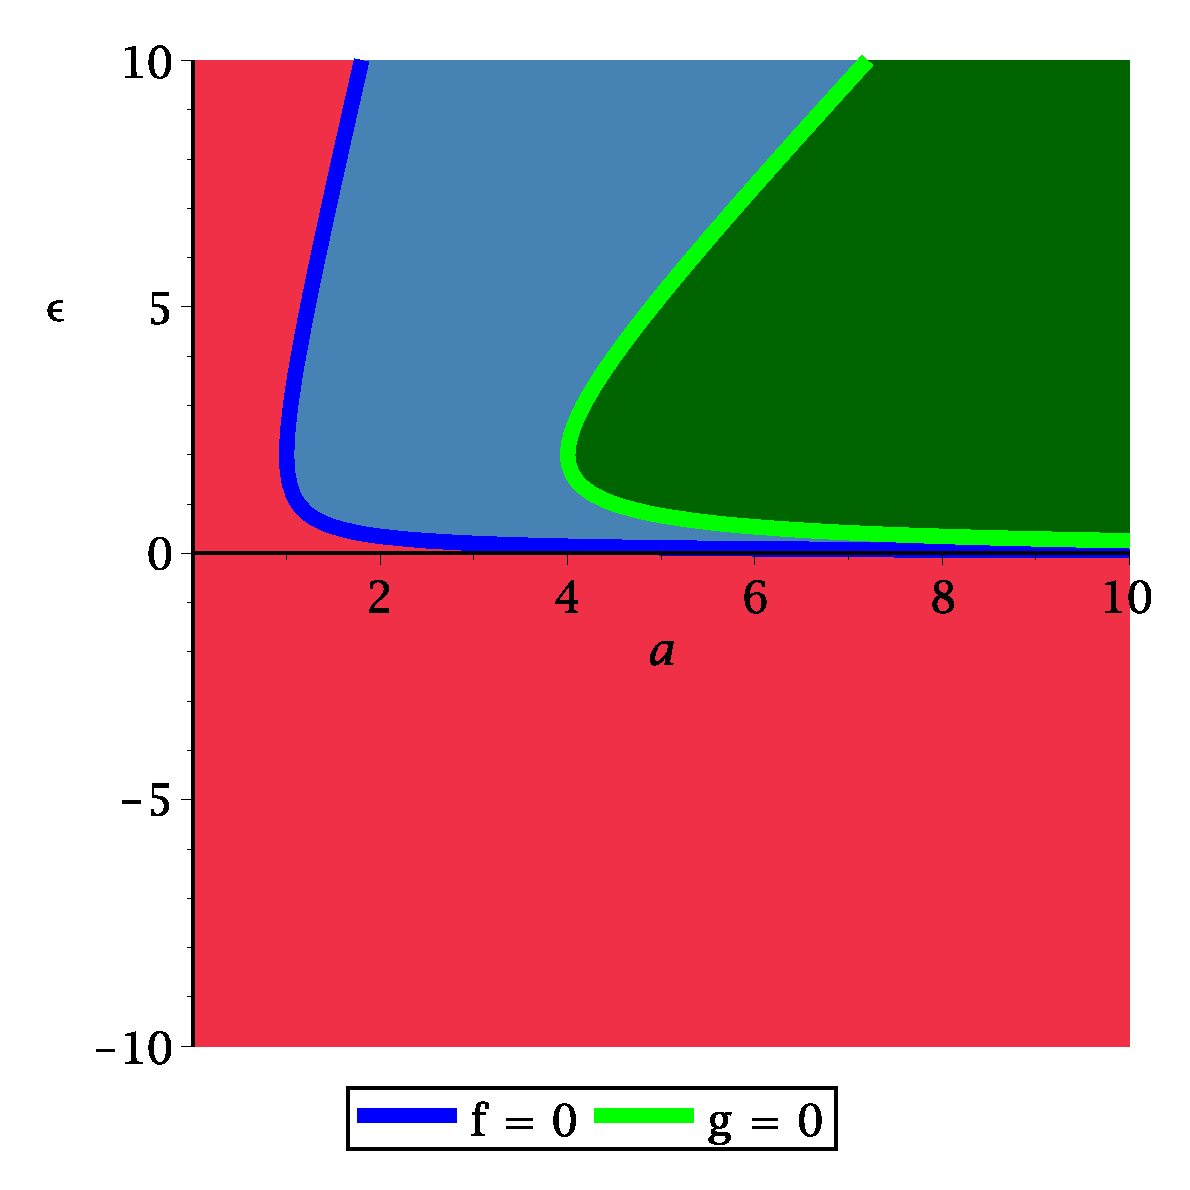
\includegraphics[width=0.5\linewidth]{Images/ex5-fg.eps}
  \caption{Gràfiques de les equacions $f=0$ i $g=0$}
  \label{ex5fg}
\end{figure}
Com podem observar a la figura \ref{ex5fg}, en la regió vermella tenim 4 punts crítics, en la regió blava 2 i en la verda 0. En les corbes blava i verda, tenim 3 i 1 equilibris respectivament.

En la regió vermella, els equilibris si $\varepsilon>-2$, $z_-^1$ i $z_+^2$ són selles i $z_+^1$ i $z_-^2$ nodes (inestable i estable, respectivament). Si $\varepsilon<-2$, $z_+^1$ i $z_-^2$ són selles i $z_-^1$ i $z_+^2$ nodes (estable i inestable, respectivament). Per $\varepsilon = -2$, $z_+^1=z_+^2=(\frac{1}{2\sqrt{a}},\frac{2}{3})$ i $z_-^1=z_-^2=(-\frac{1}{2\sqrt{a}},\frac{2}{3})$ amb valors propis $\{0,\mp 24\sqrt{a}\}$. Una de les dues varietats és atractora per un punt, i repulsora per a l'altre. Estudiant el camp sobre la varietat central, veiem que en ambdós casos comença amb sèrie amb $128a^2 z^2+\cdots$ (un cop havent centrat el punt a l'origen, és a dir $z\simeq 0)$. Per tant, tenim en ambdós casos un sella-node. Deduïm doncs que tenim una bifurcació transcrítica en la corba $\varepsilon = -2$ perquè dos parelles de punts xoquen i s'intercanvien l'estabilitat.

En la regió blava, l'estabilitat dels punts $z_\pm^2$ és la mateixa que en la regió vermella quan $\varepsilon > -2$. Finalment en les dues corbes $f=0$ i $g=0$, on els punts co\lgem isonen, tenim en ambdós casos un valor propi 0 i estudiant el camp sobre la seva corresponent varietat central deduïm que són selles nodes.

A continuació presentem els diagrames de bifurcació per a diverses seccions $a=\mathrm{const}$. En els següents gràfics la línia contínua representa el punt $z_+^1$; la discontínua amb punts, el punt $z_-^1$; la discontínua amb ratlles, el punt $z_+^2$, i la discontínua amb punts i ratlles, el punt $z_-^2$.

\begin{figure}[!ht]
  \captionsetup[subfigure]{justification=centering}
  \centering
  \begin{subfigure}[b]{0.4\linewidth}
    \centering
    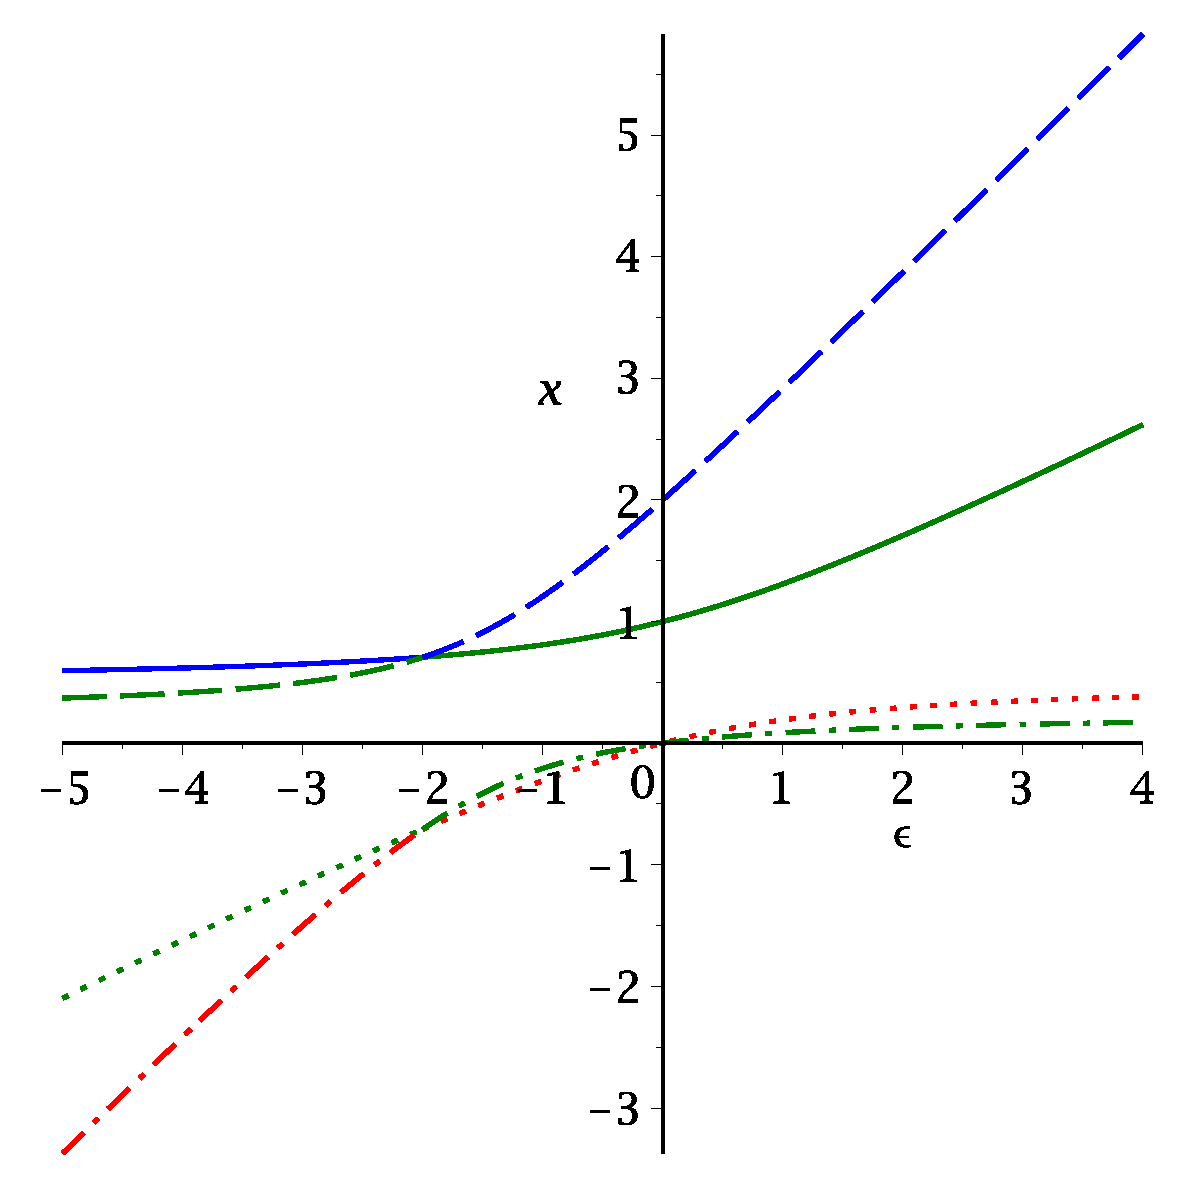
\includegraphics[width=\linewidth]{Images/ex5-a05x.eps}
    \caption{Gràfic $\varepsilon - x$}
  \end{subfigure}
  \hfill
  \begin{subfigure}[b]{0.4\linewidth}
    \centering
    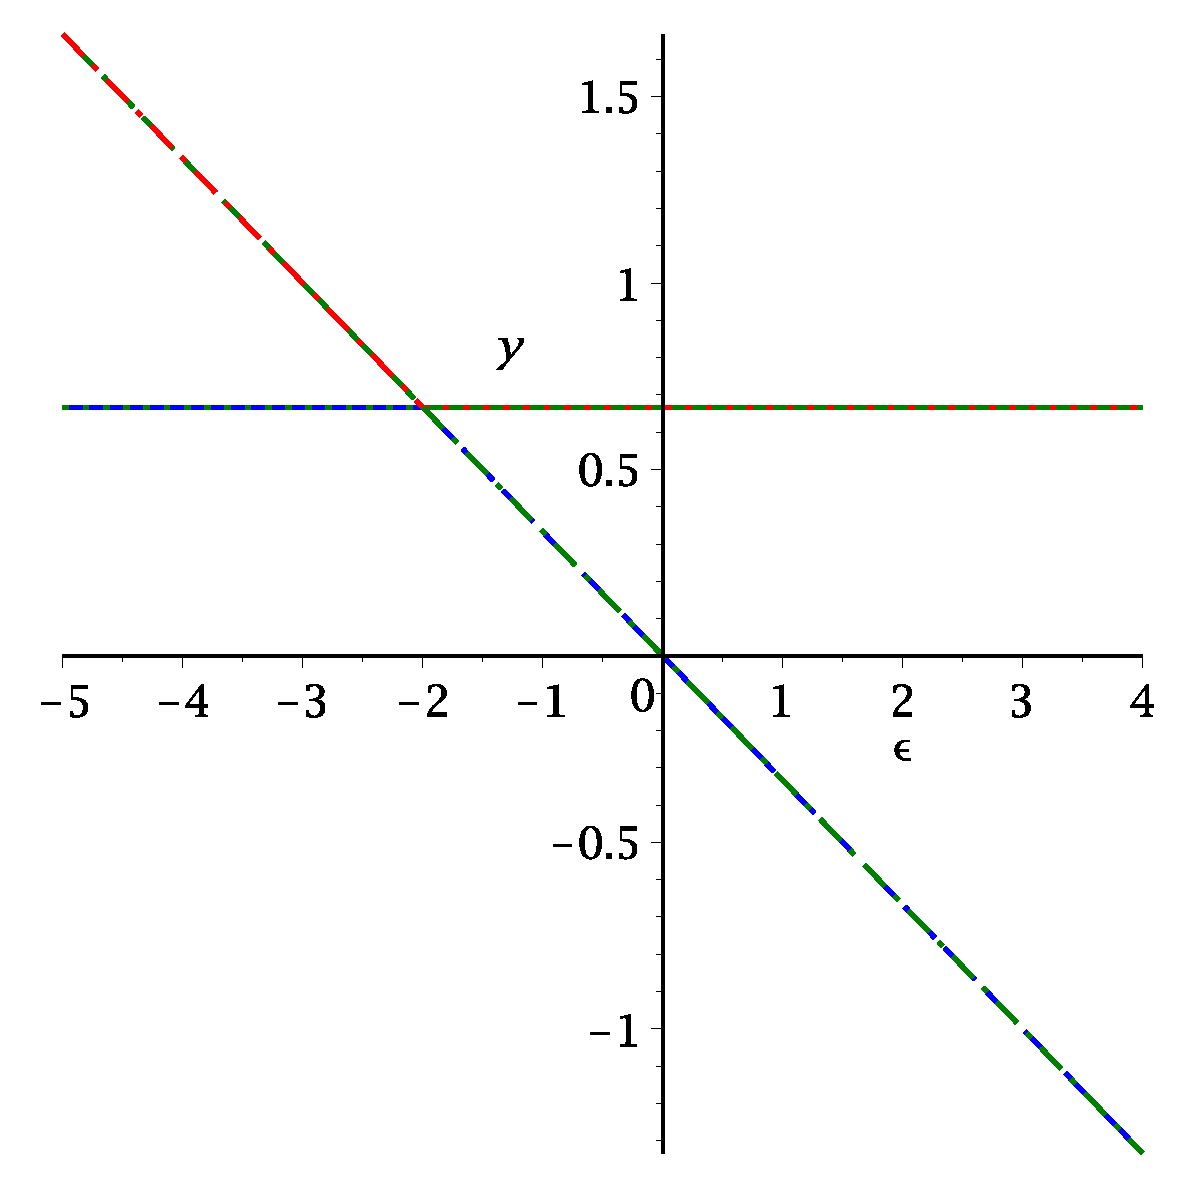
\includegraphics[width=\linewidth]{Images/ex5-a05y.eps}
    \caption{Gràfic $\varepsilon - y$}
  \end{subfigure}
  \caption{Diagrama de bifurcació dels punts d'equilibri quan $a=1/2$}
\end{figure}
\newpage
Pels següents gràfics ometrem el diagrama de les $y$, ja que sempre és de la mateixa forma.

\begin{figure}[!ht]
  \captionsetup[subfigure]{justification=centering}
  \centering
  \begin{subfigure}[b]{0.49\linewidth}
    \centering
    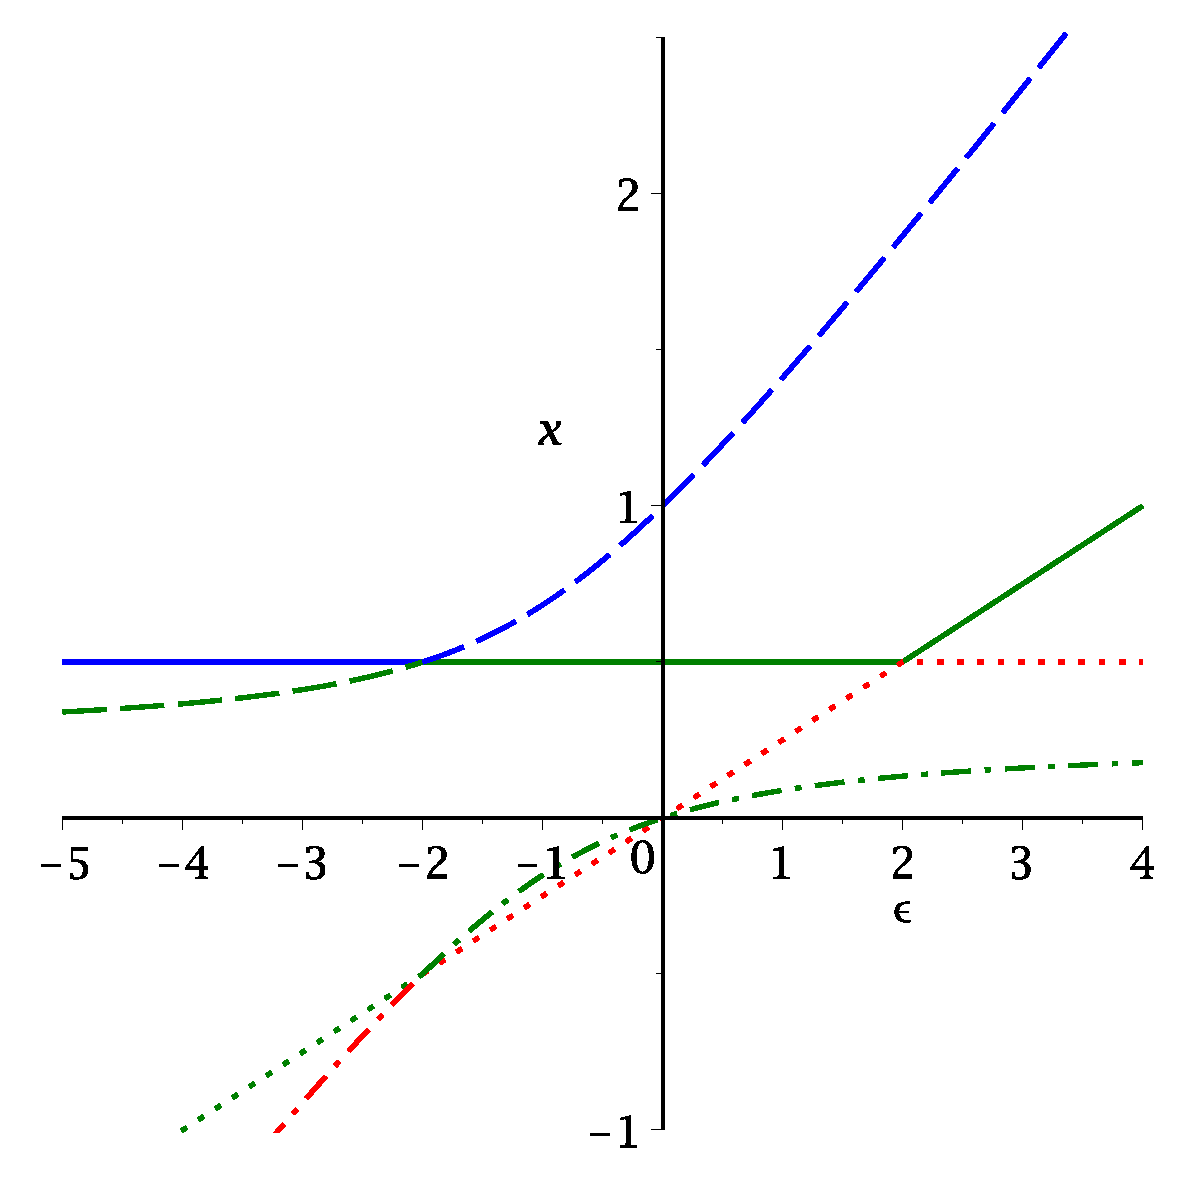
\includegraphics[width=\linewidth]{Images/ex5-a1.eps}
    \caption{Diagrama de bifurcació dels punts d'equilibri quan $a=1$}
  \end{subfigure}
  \hfill
  \begin{subfigure}[b]{0.49\linewidth}
    \centering
    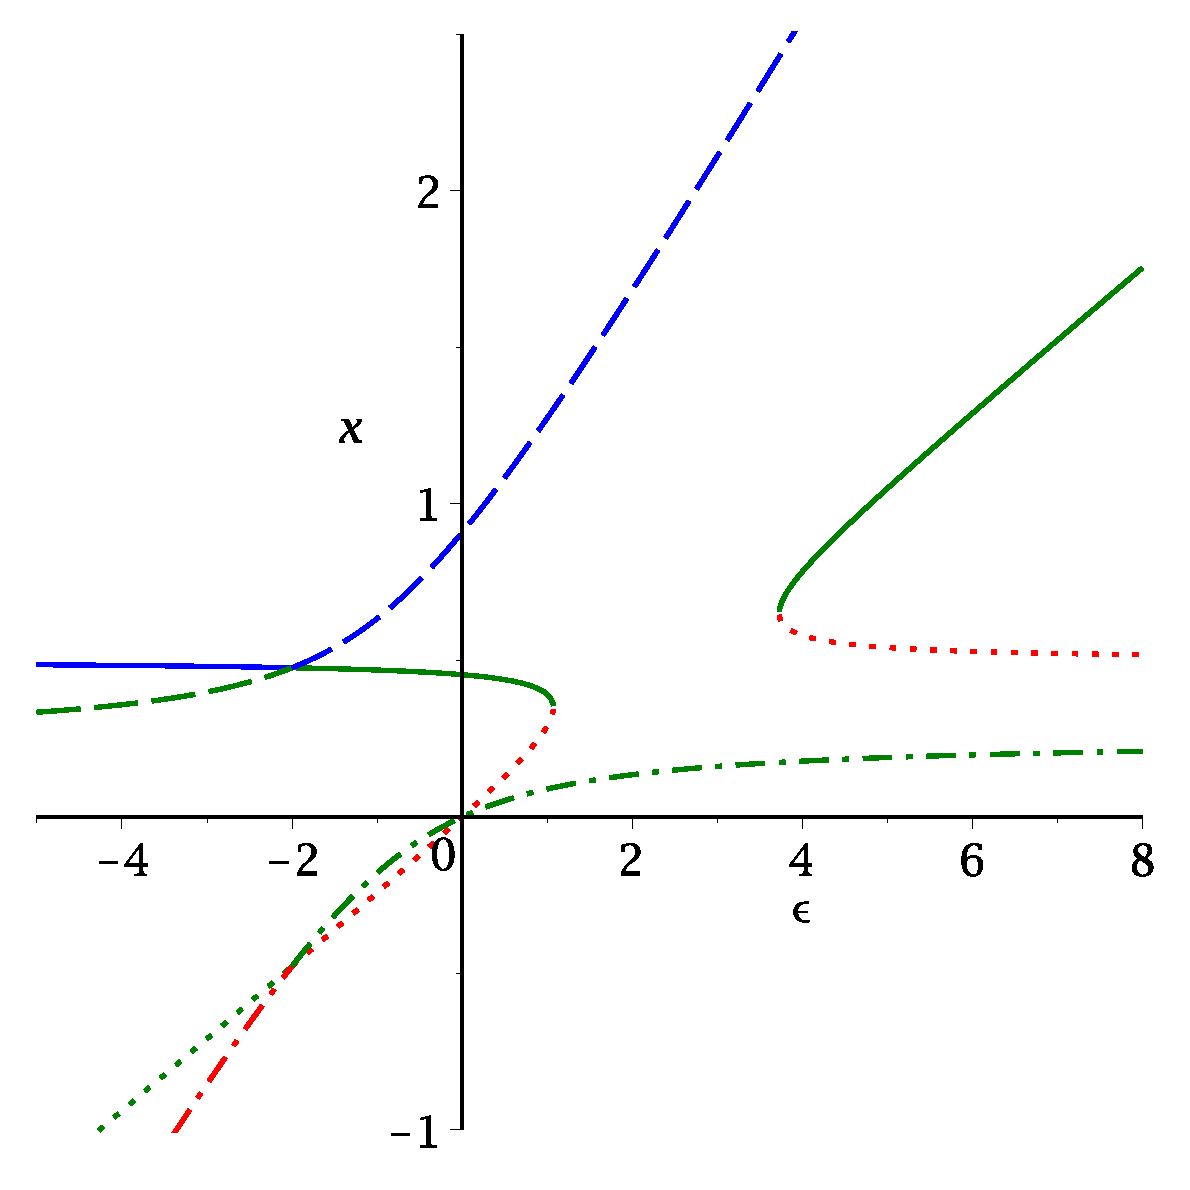
\includegraphics[width=\linewidth]{Images/ex5-a2.eps}
    \caption{Diagrama de bifurcació dels punts d'equilibri quan $a=2$}
    \label{fig2}
  \end{subfigure}
  \\
  \centering
  \begin{subfigure}[b]{0.49\linewidth}
    \centering
    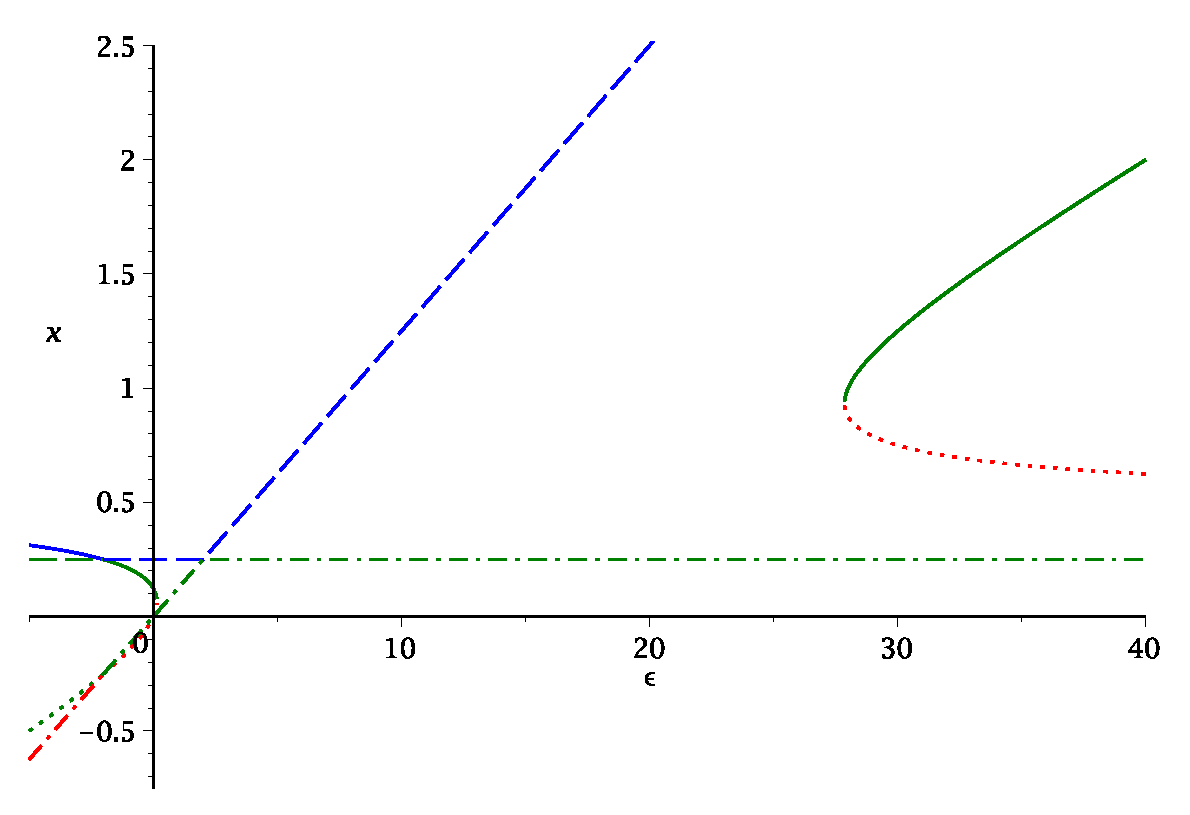
\includegraphics[width=\linewidth]{Images/ex5-a4.eps}
    \caption{Diagrama de bifurcació dels punts d'equilibri quan $a=4$}
  \end{subfigure}
  \hfill
  \begin{subfigure}[b]{0.49\linewidth}
    \centering
    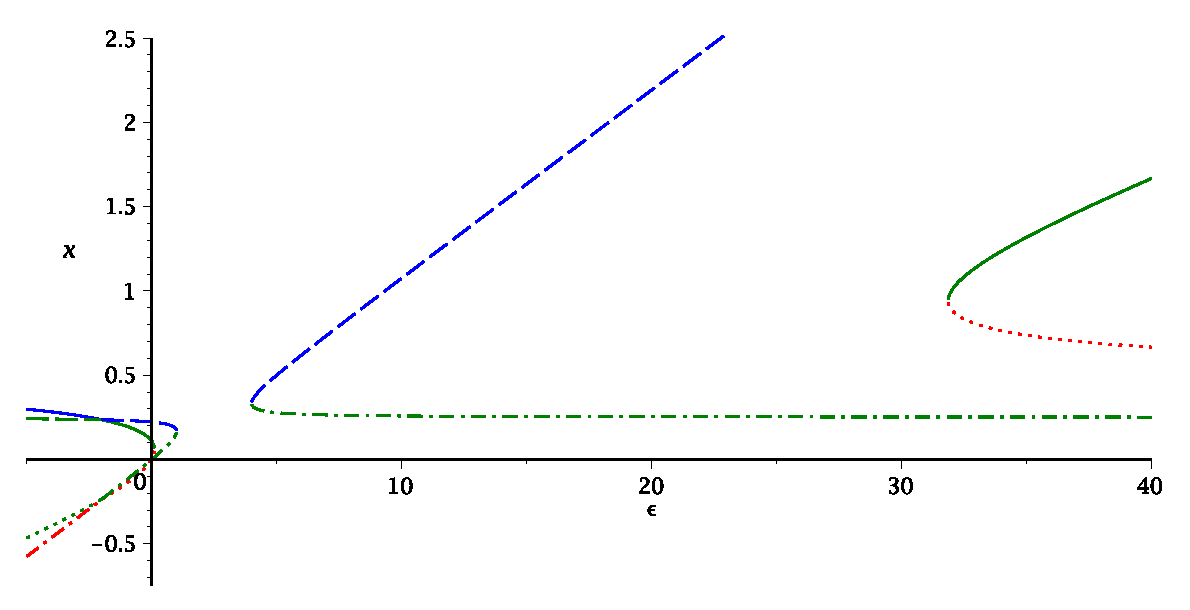
\includegraphics[width=\linewidth]{Images/ex5-a45.eps}
    \caption{Diagrama de bifurcació dels punts d'equilibri quan $a=4.5$}
  \end{subfigure}
\end{figure}

\cleardoublepage
\section*{Exercici 6}
Considerem el sistema diferencial:
\begin{equation}\label{sis6}
  \left\{
  \begin{aligned}
    x' & =-3x(28x^2-46xy+56y^2-x-122y+28) \\
    y' & =y(126x^2-92xy+42y^2-3x-122y+42)
  \end{aligned}
  \right.
\end{equation}
Volem estudiar l'estabilitat dels equilibris al primer quadrant. Aquests són els següents:
\begin{align*}
  p_1 & =(0,0)                                               & \sigma(D\vf{X}(p_1)) & =\{42, -84\}                                                                                        \\
  p_2 & =\left(0,\frac{61}{42}-\frac{\sqrt{1947}}{42}\right) & \sigma(D\vf{X}(p_2)) & =\left\{-\frac{1957}{21}+\frac{61\sqrt{1957}}{21}, \frac{1957}{21}-\frac{61\sqrt{1957}}{21}\right\} \\
  p_3 & =\left(0,\frac{61}{42}+\frac{\sqrt{1947}}{42}\right) & \sigma(D\vf{X}(p_3)) & =\left\{\frac{1957}{21}+\frac{61\sqrt{1957}}{21},-\frac{1957}{21}-\frac{61\sqrt{1957}}{21}\right\}  \\
  p_4 & =(2,3)                                               & \sigma(D\vf{X}(p_4)) & =\{684\ii, -684\ii\}
\end{align*}

Per tant, els tres primers punts són hiperbòlics amb retrat de fase local de sella tots tres. Pel quart, notem que a partir de la integrabilitat de Darboux la funció $$H = xy^2\left(-84x^2+92xy-84y^2+3x+244y-84\right)$$ és una integral primera polinomial i, per tant, el sistema és integrable. Així que el punt $(2, 3)$ és un centre.

\newpage
\section*{Exercici 7}
Considerem el sistema diferencial:
\begin{equation}\label{sis7}
  \left\{
  \begin{aligned}
    x' & =y                          \\
    y' & =\beta_1+\beta_2x + x^2 +xy
  \end{aligned}
  \right.
\end{equation}
amb $\beta_1,\beta_2\in\RR$. Se'ns demana estudiar quan obtindrem una bifurcació de Hopf. Per això estaria bé conèixer l'estabilitat dels equilibris segons $\beta_1$ i $\beta_2$.

Suposem d'entrada ${\beta_2}^2\geq 4\beta_1$, perquè si no el sistema no té equilibris. En aquest cas, aquests juntament amb els seus valors propis són els següents:
\begin{align}\label{ex7-vaps}
  z_+ & =\left(-\frac{\beta_2}{2}+\frac{\sqrt{{\beta_2}^2-4\beta_1}}{2},0\right)\quad \sigma(D\vf{X}(z_+))=\left\{-\frac{\beta_2}{4}+\frac{\sqrt{{\beta_2}^2-4\beta_1}}{4}\pm\frac{\sqrt{f(\beta_1,\beta_2)}}{4}\right\} \\
  z_- & =\left(-\frac{\beta_2}{2}-\frac{\sqrt{{\beta_2}^2-4\beta_1}}{2},0\right)\quad \sigma(D\vf{X}(z_-))=\left\{-\frac{\beta_2}{4}-\frac{\sqrt{{\beta_2}^2-4\beta_1}}{4}\pm\frac{\sqrt{g(\beta_1,\beta_2)}}{4}\right\}
\end{align}
on:
\begin{align*}
  f(\beta_1,\beta_2)=2{\beta_2}^2-4\beta_1-2\beta_2\sqrt{{\beta_2}^2-4\beta_1}+16\sqrt{{\beta_2}^2-4\beta_1} \\
  g(\beta_1,\beta_2)=2{\beta_2}^2-4\beta_1+2\beta_2\sqrt{{\beta_2}^2-4\beta_1}-16\sqrt{{\beta_2}^2-4\beta_1}
\end{align*}

Comencem l'estudi suposant que els dos punts són iguals, és a dir que ${\beta_2}^2=4\beta_1$. Si $\beta_2=\beta_1=0$, l'origen és un \emph{cusp}, pel teorema de classificació de punts nilpotents. Ara suposem $\beta_2\ne 0$ i passem el sistema a la seva forma de Jordan:
\begin{equation}
  \left\{
  \begin{aligned}
    x' & =X(x,y,\vf\beta)                     \\
    y' & =-\frac{\beta_2}{2}y+Y(x,y,\vf\beta)
  \end{aligned}
  \right.
\end{equation}
on $\vf\beta=(\beta_1,\beta_2)$ i $X$ i $Y$ tenen sèrie de Taylor començant per ordre 2. Fent càlculs i usant el teorema de classificació de punts semihiperbòlics resulta que obtenim un sella-node.

Ara suposem que ${\beta_2}^2>4\beta_1$ i observem que: $$f(\beta_1,\beta_2)={\left(\beta_2-\sqrt{{\beta_2}^2-4\beta_1}\right)}^2+16\sqrt{{\beta_2}^2-4\beta_1}> 0$$
Per tant, $z_+$ sempre té valors propis reals i el seu producte és $-\sqrt{{\beta_2}^2-4\beta_1}< 0$. Per tant, aquest punt sempre és una sella.

Centrem-nos ara amb $z_-$. Fent càlculs deduïm que els valors propis en aquest punt si s'anu\lgem en només ho fan quan ${\beta_2}^2=4\beta_1$. D'altra banda, la corba $g = 0$ té solució i és la corba que ``zigzagueja'' en la figura \ref{ex7z-} pintada de color blau cel en el dos quadrants superiors i de color rosa en els dos quadrants inferiors. Per tant, hi haurà valors pels quals els valors propis seran imaginaris. Quan la part real d'aquests valors propis sigui diferent de zero, podrem aplicart Hartman. Per tant, ens interessa estudiem quan la part real és igual a zero. Mirant l'equació \eqref{ex7-vaps} deduïm que això passa si i només si $\beta_1=0$ i $\beta_2\leq 0$. Reescalant convenientment el sistema, observem que el podem escriure en la seva forma de Jordan real:
\begin{equation*}
  \left\{
  \begin{aligned}
    x' & =\sqrt{-\beta_2}y                                    \\
    y' & =-\sqrt{-\beta_2}x + \frac{x^2}{\sqrt{-\beta_2}} +xy
  \end{aligned}
  \right.
\end{equation*}
El primer coefficient de Lyapunov d'aquest sistema és $-\frac{1}{4\beta_2}>0$. Per tant, tenim un focus repulsor (feble, perquè te part real nu\lgem a).

Finalment falta estudiar el comportament en la corba $g=0$. El producte dels valors propis és sempre $\sqrt{{\beta_2}^2-4\beta_1}> 0$. Per tant només podem tenir nodes. Fent càlculs, es veu que la suma d'aquests és negativa si $\beta_2>0$ i positiva si $\beta_2<0$. Per tant, si $\beta_2>0$ tenim un node atractor; si $\beta_2<0$, una node repulsor.

El diagrama següent mostra un resum de tot l'estudi fet. A l'àrea blanca no està definit el punt d'equilibri.
\begin{figure}[ht]
  \centering
  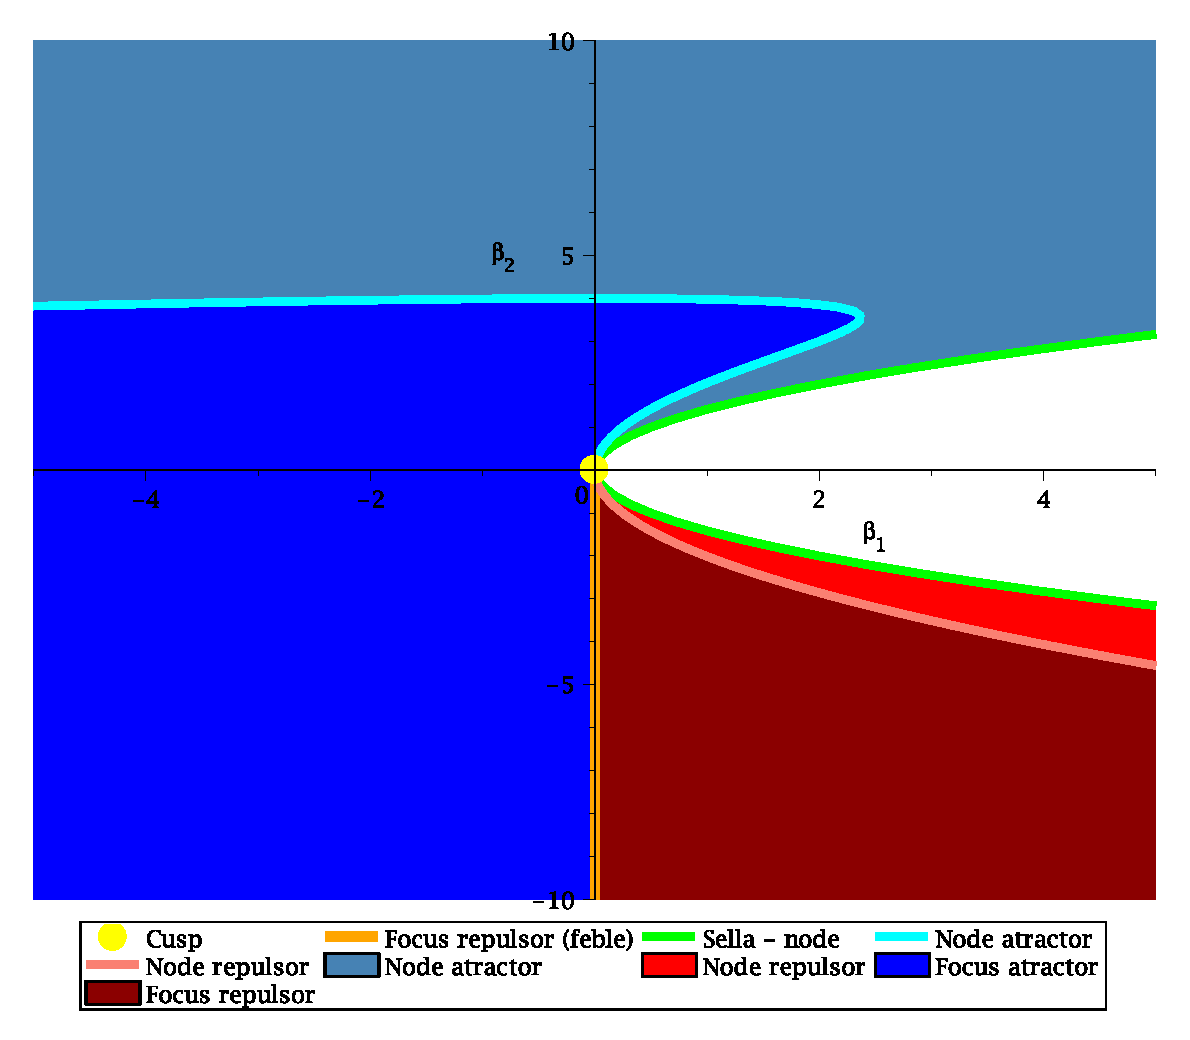
\includegraphics[width=\linewidth]{Images/ex7-diag2.eps}
  \caption{Gràfic del comportament qualitatiu del punt $z_-$}
  \label{ex7z-}
\end{figure}

Tindrem, doncs, una bifurcació de Hopf al variar $\beta_1\sim 0$ quan $\beta_2<0$, d'on surtirà un únic cicle límit.
\end{document}